\section{Zielsetzung}
\label{sec:Zielsetzung}
Ziel dieses Experiments ist es, mittels Röntgenreflektivität die Strukturmerkmale
eines Polystyrolfilms auf einem Siliziumwafer zu analysieren. Die Analyse umfasst die 
Bestimmung der Dichte, Rauhigkeit und Schichtdicke des Films. Die gemessenen Daten liefern
Informationen über die Materialeigenschaften, die in der Mikroelektronik von großer Bedeutung sind.
Zudem soll ermittelt werden, wie effektiv Röntgenreflektivität zur Untersuchung von Grenzflächen auf festen 
und flüssigen Substraten eigesetzt werden kann.


\section{Theorie}
\label{sec:Theorie}
Röntgenstrahlung ist eine elektromagnetische Strahlung, die sich durch ihre hohe Energie und kurze 
Wellenlänge \(\lambda\) (0.01 bis 10 Nanometer) auszeichnet. Die Strahlung entsteht hauptsächlich durch 
Bremsstrahlung und durch charakteristische Röntgenstrahlung.

\subsection{Strahlungsarten}
Bremsstrahlung entsteht, wenn schnelle Elektronen in der Nähe von Atomkernen abgelenkt werden und dabei Energie
in Form von Photonen abgeben. Diese werden in eine Röntgenröhre beschleunigt und auf ein Metalltarget geschossen.
Beim Aufprall werden sie abgebremst und emittieren dabei Röntgenstrahlung. Diese Strahlung ist in dem Röntgenspektrum in
\ref{fig:Abbildung 1} mit dem kontinuierlichen Energiespektrum zu identifizieren.
Die charakteristische Röntgenstrahlung entsteht durch Übergänge von Elektronen in den Schalen von Atomen. Wenn Elektronen 
aus den inneren Schalen eines Atoms herrausgeschossen werden, füllen Elektronen aus höheren Schalen die frei gewordenen Plätze.
Während des Übergangs von Elektronen aus höheren Schalen in die freien Plätze der inneren Schalen wird die Differenz der
Energieniveaus der beiden Schalen in Form von Röntgenphotonen freigesetzt. Diese Energieemission entsteht, weil die Elektronen
beim Herabfallen auf ein niedrigeres Energieniveau überschüssige Energie abgeben, die als Röntgenstrahlung sichtbar wird. Die Strahlung 
zeigt ein diskretes Energiespektrum, das von den spezifischen Energieniveaus der Elektronen in den Atomen des Targets abhängt.


\begin{figure}
    \includegraphics[width=\textwidth]{bilder/Röntgenspektrum.jpg}
    \caption{Schematischer Abbildung des Röntgenspektrums}
    \label{fig:Abbildung 1}
\end{figure}

\subsection{Verhalten an Grenzflächen}
Beim Einfall von Röntgenstrahlung auf eine glatte Grenzfläche wird diese durch den Brechungsindex des Mediums beeinflusst.
Der komplexe Brechungsindex wird beschrieben durch:
\begin{equation}
    n=1-\delta+i\beta
\end{equation}
Dabei ist der Parameter \(\delta\) eine sehr kleine Korrekturgröße im Bereich von $10^{-6}$
und gibt an, wie stark die Phasenverschiebung der Röntgenstrahlung beim Durchgang durch das Medium ist.
Diese Korrektur ist dimensionslos. Der imaginäre Teil \(i\beta\) beschreibt die Absorption der Strahlung im Material.
Hierbei steht \(\beta\) für den Absorptionskoeffizienten, je größer dieser ist, desto stärker wird die Strahlung absorbiert.

\begin{figure}
    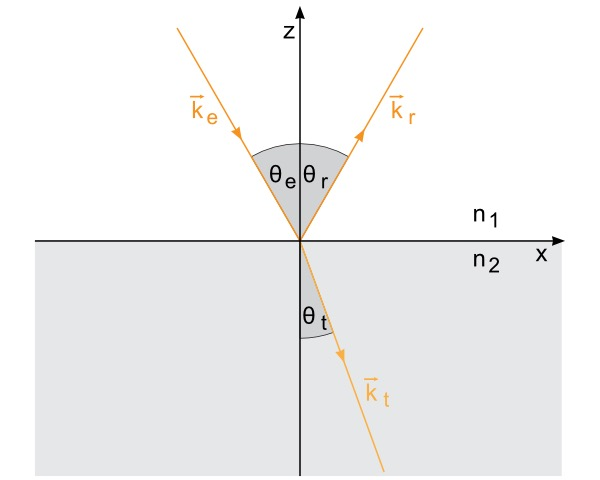
\includegraphics[width=\textwidth]{bilder/Reflexion.jpg}
    \caption{Skizze zum Verhalten elektromagnetischer Strahlung an einer Grenzschicht zwischen zwei Medien}
    \label{fig:Abbildung 2}
\end{figure}
In \ref{fig:Abbildung 2} sind die Wellenvektoren der einfallenden $\vec{k}_e$, reflektierten $\vec{k}_r$ und der
transmittierten $\vec{k}_t$ Wellen sowie die entsprechenden Winkel zur Ebene $(\theta_e,\theta_r,\theta_t)$ dargestellt.
Das Snellius-Brechungsgesetzt besagt:
\begin{equation}
    n_1cos(\theta_e)=n_2cos(\theta_a)
\end{equation}
Wobei $\theta_a$ der Ausfallswinkel ist und $\theta_e=\theta_r$ gilt.    
Die Fresnel-Gleichungen beschreiben die Amplitudenverhältnisse von senkrecht und parallel polarisiertem Licht
an einer Grenzfläche. Bei Röntgenstrahlung sind diese Verhältnisse für parallel und senkrecht polarisierten Anteil nahezu 
identisch. Das liegt daran, dass die die Brechungsindizes kaum Unterschiede aufweisen. 
Der Reflexionskoeffizient \(r\) gibt das Verhältnis der Amplitude der reflektierten Welle zur Amplitude der einfallenden Welle an. 
Er beschreibt, wie viel der einfallenden Welle an der Grenzfläche reflektiert wird. Der Betrag von \(r\) kann zwischen 0 und 1
liegen, wobei 0 bedeutet, dass keine Reflexion stattfindet und 1 bedeutet, dass die gesamte Welle reflektiert wird.
Der Transmissionskoeffizient \(t\) gibt das Verhältnis der Amplitude der transmittierten Welle zur Amplitude der einfallenden Welle an.
Er beschreibt, wie viel der einfallenden Welle die Grenzfläche durchdringt und in das zweite Medium gelangt. Auch hier kann der Betrag 
zwischen 0 und 1 liegen, wobei 0 bedeutet, dass keine Transmission stattfindet und 1 bedeutet, dass die gesamte Welle durchgelassen wird.
Diese Koeffizienten sind wie folgt definiert:
\begin{equation}
    r=\frac{n_1sin(\theta_i)-n_2sin(\theta_t)}{n_1sin(\theta_i)+n_2sin(\theta_t)}
\end{equation}
\begin{equation}
    t=\frac{2n_1sin(\theta_i)}{n_1sin(\theta_i)+n_2sin(\theta_t)} 
\end{equation}
Wenn das erste Medium Vakuum ist (n=1), tritt bei einem kritischen Winkel $\theta_c$ Totalreflexion auf, da der Brechungsindex von Materie für
Röntgenstrahlung immer kleiner als 1 ist. Dieser kritische Winkel kann näherungsweise durch folgende Gleichung bestimmt werden:
\begin{equation}
    \theta_c = \sqrt{2\delta} = \lambda \sqrt{\frac{r_e \rho}{\pi}}
\end{equation}    
dabei sind $\lambda$ die Wellenlänge der Röntgenstrahlung, \(r_e\) der klassische Elektronenradius und $\rho$ die Elektronendichte des Materials.
Für die Reflektivität \(R\), die das Verhältnis der Intensitäten der reflektierten und der einfallenden Welle beschreibt gilt:
\begin{equation}
    R=|r|^2
\end{equation}
Unter der Annahme dass $\theta_i>3\theta_c$ gilt:
\begin{equation}
    R=(\frac{\theta_c}{2\theta_i})^4
\end{equation}    


\cite{sample}
